\chapter{Activating an image}
\label{activate}
\minitoc
After a logical extend (an image) has been created from a physical
extend there are in principal four possibilities to activate the
image:

\begin{enumerate}
	\item In case of a \textbf{local accessable system harddisk}, the image
          can be installed by dumping (dd) the image file on a previously
          created partition on this disk. To activate the system a boot
          manager like grub or lilo can be used
	\item In case of a \textbf{network enabled system} (netboot client)
          the image can be installed via a special boot image.
          The boot image which serves as initial ramdisk (initrd) and
          the appropriate kernel are downloaded from a network service.
          The linux kernel automatically calls a program named
          \textbf{linuxrc} which takes over all tasks needed to download
          and install the system image. The installation can be done
          persistently on disk or temporary into the RAM of the machine.
	\item In case of a \textbf{para virtualized target system} like Xen,
          the image can be be installed by copying the image file on the
          target system. To activate the virtual system a configuration
          must be provided which points to the image in some way. One
          possibility is to use a loop mounted location.
	\item In case of a \textbf{full virtualized target system} like VMware,
          or QEMU the image represents a virtual disk as file which can
          be \textit{played} by the virtualisation system.
\end{enumerate}

\section{The KIWI netboot image}

The KIWI netboot image can be used to install an operating system image to
a network client. To establish communication with the client a
boot server infrastructure including the following services is required:

\begin{itemize}
	\item DHCP server to give the client an IP address
	\item TFTP server to allow file transfer from/to the client 
\end{itemize}

\index{boot images|(}
\index{NBs!booting|(}
\subsection{The Boot Process of a netboot System}
\label{NBbootprocess}
To understand how to use the operating system image with the netboot
image, a short description of the netboot client is useful. The
following diagram shows the simplified boot process of a netboot
client.

\begin{figure}[h]
\centering
\includegraphics[scale=0.5]{pictures/nbboot.eps}
\caption{The Boot Process of a netboot client}
\label{fig:architecture}
\end{figure}

The most important point is to understand the cooperation between
the initial boot image \textbf{initrd.gz} and the intrinsic operating system
image. If the system is able to boot via a network, it will load the kernel
and the compressed boot image from the network. The \textit{brain} of the
boot image is the \textbf{linuxrc} script, which does all the
stuff controlled by an image configuration file also obtained from the
network. The major task is to download and activate the operating system
image. The boot image is exchanged for the operating system image to be
activated. The following overview describes the steps that take
place when the netboot client is booted:

\begin{itemize}
\item Via PXE network boot or boot manager (GRUB), the client boots the
      initrd (initrd.gz) that it receives from the TFTP server. If no PXE
      boot is possible, the client tries to boot from the hard
      disk, if accessible.
\item Running \textbf{linuxrc} starts the process described below.
\end{itemize}

\begin{enumerate}
	\item The required file systems to receive system data are mounted.
          Example: \textbf{proc} file system.
	\item Network support is activated. A default list of modules is
		  used and are tried one after the other. The module is loaded
		  using \textit{modprobe}. Any dependencies to other modules are
          cleared at that time.
	\item The network interface is set up via DHCP. After the interface has
          been established, the DHCP variables are exported into the file
          \textit{/var/lib/dhcpcd/dhcpcd-eth0.info} and the contents of
          DOMAIN and DNS are used to generate a \textit{/etc/resolv.conf}.
	\item The TFTP server address is acquired. During this step, a check
          is first made to determine whether the host name
          \textbf{tftp.\$DOMAIN} can be resolved. If not, the DHCP
          server is used as the TFTP server. For more infomation about the
          TFTP servers structure, refer to Section \ref{section:tftpstruct}
	\item The configuration file is loaded from the server directory
          \textit{/var/lib/tftpboot/KIWI} via TFTP. At this point, the client
          expects the file:

          \begin{Command}{8cm}
          config.$<$MAC Address$>$
          \end{Command}

          If this file is not available and cannot be loaded, it means this
          is a new client that can be immediately registered. A new client is
          registered by uploading a control file to the TFTP servers upload
          directory: \textit{/var/lib/tftpboot/upload}. After the upload, the client
          branches off into a loop in which the following steps are taken:

          \begin{itemize}
          \item the DHCP lease file is renewed (\textit{dhcpcd -n}).
          \item a new attempt is made to load the file
                config.$<$MAC address$>$ from the TFTP server.
          \item if the file does not exist, there is a 60-second wait
                period before a new run begins.
          \end{itemize}

          If the configuration file does load, it contains data on
          image, configuration, synchronization, or partition parameters.
          For more infomation about the file format of the configuration file,
          refer to Section \ref{section:confmac}.

	\item The PART: line in the configuration is analyzed. If there is a
          PART line in the configuration file, the following analysis
          takes place:
          \begin{itemize}
          \item A check is made using the image version to see whether any
                local system needs to be updated. If not, local boot process
                continues immediately. No image download occurs.
          \item No system or update required: client hard disk is
                partitioned.
          \end{itemize}
	\item Indicated images are downloaded with multicast TFTP.
	\item Checksums checked. Repeat download if necessary.
	\item The CONF: line is evaluated. All the indicated files are loaded
          from the TFTP server and stored in a \textit{/config/} path.
	\item Terminate all the user-land processes based on the boot image
          (dhcpcd -k).
	\item operating system image is mounted.
	\item The configuration files stored in \textit{/config/...} are copied
          into the mounted operating system image.
	\item The system switches to the mounted operating system image. The root
          file system is converted to the operating system image via
          \textbf{pivot\_root}. All the required configuration files are
          now present, because they had been stored in the operating system
          image or have been downloaded via TFTP.
	\item The boot image is unmounted using an \textbf{exec umount} call.
	\item At termination of linuxrc or the exec call, the kernel initiates
          the \textbf{init} process that starts processing the boot
          scripts as specified \textbf{/etc/inittab}, for example,
          to configure the network interface.
\end{enumerate}

\index{boot server|(}
\subsection{TFTP Server Structure}
\label{section:tftpstruct}
The TFTP server directory structure is divided into the following main areas

\begin{itemize}
\item \textbf{Image configurations}\\
      The \textit{/var/lib/tftpboot/KIWI/}~ directory contains the various
      \textit{config.$<$MAC Address$>$} image configuration files.
\item \textbf{Configuration files}\\
      The \textit{/var/lib/tftpboot/KIWI/$<$MAC Address$>$/}~ directory
      contains the various system configuration files, such as xorg.conf.
\item \textbf{Boot files}\\
      The \textit{/var/lib/tftpboot/boot/}~ directory is where the initrd.gz,
      and the kernel to boot are kept.
\item \textbf{PXE second stage boot loader(s)}\\
      The \textit{/var/lib/tftpboot/}~ directory is where the boot loaders
      for PXE are kept (pxelinux.0,mboot.c32)
\item \textbf{PXE configuration file}\\
      The \textit{/var/lib/tftpboot/pxelinux.cfg}~ directory is where
      the PXE configuration file is kept.
\item \textbf{Image files and checksums}\\
      The \textit{/var/lib/tftpboot/image/}~ directory is where all the image
      files and their checksums are kept.
\item \textbf{Upload area}\\
      The directory \textit{/var/lib/tftpboot/upload/}~ is the directory into
      which the \textit{hwtype.$<$MAC Address$>$} files for registering
      new netboot clients are uploaded.
\end{itemize}

%\newpage

\index{configuration files!config.<MAC Address>|(}
\subsection{The netboot client Configuration File}
\label{section:confmac}
This section describes the netboot client configuration file:

\begin{Command}{8cm}
	config.$<$MAC Address$>$
\end{Command}

The configuration file contains data about image, configuration,
synchronization, or partition parameters. The configuration file is
loaded from the TFTP server directory \textit{/var/lib/tftpboot/KIWI} via TFTP
for previously installed netboot clients. New netboot clients are
immediately registered and a new configuration file with the
corresponding MAC address is created. Below, find an example of a cash
register configuration file:

\begin{verbatim}
IMAGE=/dev/hda2;image/browser;1.1.1;192.168.1.1;4096
CONF=/KIWI/00:30:05:1D:75:D2/ntp.conf;/etc/ntp.conf;192.168.1.1;1024,     \
     /KIWI/00:30:05:1D:75:D2/xorg.xonf;/etc/X11/xorg.xonf;192.168.1.1;1024
PART=200;S;x,300;L;/,500;L;/opt,x;L;/home
DISK=/dev/hda
\end{verbatim}

The following format is used:

\begin{Command}{14cm}
	\textbf{IMAGE}=\underline{device;name;version;srvip;bsize;compressed},...,\\
	\textbf{SYNC}=syncfilename;srvip;bsize\\
	\textbf{CONF}=\underline{src;dest;srvip;bsize},...,
                             src;dest;srvip;bsize\\
	\textbf{PART}=\underline{size;id;Mount},...,size;id;Mount\\
	\textbf{JOURNAL}=ext3\\
	\textbf{DISK}=device
\end{Command}

\begin{itemize}
	\item \textbf{IMAGE}\\
		Specifies which image (name) should be loaded with which
		version (version) and to which storage device (device) it
		should be linked, e.g., \textbf{/dev/ram1} or
		\textbf{/dev/hda2}. The netboot client partition (device)
		\textbf{hda2} defines the root file system "/" and \texttt{hda1}
		is used for the swap partition. The numbering of the hard disk
		device should not be confused with the RAM disk device,
		where \texttt{/dev/ram0} is used for the initial RAM disk and
		can not be used as storage device for the second stage system image.
		SUSE recommends to use the device \texttt{/dev/ram1} for the
		RAM disk. If the hard drive is used, a corresponding partitioning
		must be performed.
	\item \textbf{srvip}\\
		Specifies the server IP address for the TFTP download.
		Must always be indicated, except in PART.
	\item \textbf{bsize}\\
		Specifies the block size for the TFTP download. Must always
		be indicated, except in PART. If the block size is too small
		according to the maximum number of data packages (32768),
		\textbf{linuxrc} will automatically calculate a new blocksize for
		the download.
    \item \textbf{compressed}\\
        Specifies if the image file on the TFTP server is compressed and
        handles it accordingly. To specify a compressed image download only
        the keyword \textbf{"'compressed"'} needs to be added. If compressed
        is not specified the standard download workflow is used. \textbf{Note:}
        The download will fail if you specify "'compressed"' and the image isn't
        compressed. It will also fail if you don't specify "'compressed"'
        but the image is compressed. The name of the compressed image has
        to contain the suffix \textbf{.gz} and needs to be compressed with the
        \textbf{gzip} tool. Using a compressed image will automatically
        \textbf{deactivate} the multicast download option of atftp.
	\item \textbf{CONF}\\
		Specifies a comma-separated list of source:target
		configuration files. The source (src) corresponds to the path
		on the TFTP server and is loaded via TFTP. The
		download is made to the file on the netboot client
		indicated by the target (dest).
	\item \textbf{PART}\\
		Specifies the partitioning data. The comma-separated list
		must contain the size (size), the type number (id), and the
		mount point (Mount). The size is measured in MB by default.
		Additionally all size specifications supported by the sfdisk
		program are allowed as well. The type number specifies the ID
		of the partition. Valid ID's are listed via the
		\textit{sfdisk --list-types} command. The mount specifies the
		directory the partition is mounted to.
		\begin{itemize}
			\item The first element of the list must define the swap
                  partition.
            \item The second element of the list must define the
                  \textbf{root} partition.
	        \item The swap partition must not contain a mount point.
                  A lowercase letter \textbf{x} must be set instead.
            \item If a partition should take all the space left on
                  a disk one can set a lower \textbf{x} letter as
                  size specification.
		\end{itemize}
	\item \textbf{DISK}\\
		Specifies the hard disk. Used only with PART and defines
		the device via which the hard disk can be addressed,
		e.g., \textbf{/dev/hda}.
	\item \textbf{RELOAD\_IMAGE}\\
		If set to a non-empty string, forces the configured
		image to be loaded from the server even if the image on
		the disk is up-to-date. Used mainly for debugging
		purposes, this option only makes sense on diskful
		systems.
	\item \textbf{RELOAD\_CONFIG}\\
		If set to an non-empty string, forces all config files
		to be loaded from the server. Used mainly for debugging
		purposes, this option only makes sense on diskful
		systems.
	\item \textbf{COMBINED\_IMAGE}\\
        If set to an non-empty string, indicates that the both
        image specified needs to be combined into one bootable
        image, whereas the first image defines the read-write
        part and the second image defines the read-only part.
\end{itemize}

%\newpage

\index{NBs!control file|(}
\index{configuration files!hwtype.<MAC Address>|(}
\subsection{The netboot client Control File}
\label{section:cntrlhw}
This section describes the netboot client control file:

\begin{Command}{8cm}
hwtype.$<$MAC Address$>$
\end{Command}

The control file is primarily used to set up new netboot clients. In this
case, there is no configuration file corresponding to the client
MAC address available. Using the MAC address information, the control file
is created, which is uploaded to the TFTP servers upload directory
\textit{/var/lib/tftpboot/upload}.

\section{The Xen virtual machine}
To use an image within Xen the most important point is to use
the para virtualized xen kernel within the operating system image.
While creating a xen based image \textbf{kiwi} will take care
for the correct kernel to be used.

\subsection{Activate a KIWI xen image}
To activate an image including the xen kernel the following steps
needs to be performed:

\begin{enumerate}
	\item boot the system using the command:

          \begin{Command}{9cm}
          xm create -c <xen config file>
          \end{Command}

          The xen config file will be created automatically by kiwi.
          Of course this file can be enhanced to some degree, for example
          adding the virtual network driver, etc...

    \item for more information on how to configure xen refer to\\
          http://en.opensuse.org/Installing\_Xen3
\end{enumerate}

\section{The VMware virtual machine}
VMware represents a full virtualized machine which means all components
are virtualized. This includes the storage devices as well as the
processor and all other parts of the system. An image for such a system
is in principal a virtual disk which contains the boot manager the
initrd and all other system data as one file. Kiwi is able to create
such a disk appropriate for use in QEMU and VMware (vmdk format).

\subsection{Activate a KIWI virtual disk system}
To activate such a system the user only needs to call the correct
\textit{player} application which in case of QEMU is \textbf{qemu} and
in case of VMware \textbf{vmplayer} is used.
